\documentclass{article}
\RequirePackage{amsmath}
 \usepackage{gensymb}
 \usepackage{graphicx}
 \usepackage{setspace}
 \usepackage{subcaption}
 \usepackage{geometry}
 \geometry{
 a4paper,
 left=20mm,
 right=20mm,
 bottom=25mm,
 top=25mm,
 }
%\doublespacing
 \usepackage{polynom}
\usepackage{amssymb}
\usepackage{amsthm}
 \usepackage{stfloats}
 \usepackage{float}
% \usepackage{steinmetz}
 \usepackage{bm}
\usepackage{longtable}
\usepackage{enumitem}
 \usepackage{mathtools}
 \usepackage{tikz}
\usepackage[breaklinks=true]{hyperref}
\usepackage{listings}
    \usepackage{color}                                            %%
    \usepackage{array}                                            %%
    \usepackage{longtable}                                        %%
    \usepackage{calc}                                             %%
    \usepackage{multirow}                                         %%
    \usepackage{hhline}                                           %%
    \usepackage{ifthen}                                           %%
    \usepackage{amsmath}
\DeclareMathOperator*{\Res}{Res}
\DeclareMathOperator*{\equals}{=}
\hyphenation{op-tical net-works semi-conduc-tor}
                                %%

\lstset{
frame=single, 
breaklines=true,
columns=fullflexible
}

\begin{document}

\newtheorem{theorem}{Theorem}[section]
\newtheorem{problem}{Problem}
\newtheorem{proposition}{Proposition}[section]
\newtheorem{lemma}{Lemma}[section]
\newtheorem{corollary}[theorem]{Corollary}
\newtheorem{example}{Example}[section]
\newtheorem{definition}[problem]{Definition}
\newcommand{\BEQA}{\begin{eqnarray}}
\newcommand{\EEQA}{\end{eqnarray}}
\newcommand{\define}{\stackrel{\triangle}{=}}
\newcommand*\circled[1]{\tikz[baseline = (char.base)]{ \node[shape=circle,draw,inner sep=2pt] (char) {#1}; }}
\providecommand{\mbf}{\mathbf}
\providecommand{\pr}[1]{\ensuremath{\Pr\left(#1\right)}}
\providecommand{\qfunc}[1]{\ensuremath{Q\left(#1\right)}}
\providecommand{\sbrak}[1]{\ensuremath{{}\left[#1\right]}}
% \providecommand{\lsbrak}[1]{\ensuremath{{}\left[#1\right.}}
% \providecommand{\rsbrak}[1]{\ensuremath{{}\left.#1\right]}}
% \providecommand{\brak}[1]{\ensuremath{\left(#1\right)}}
% \providecommand{\lbrak}[1]{\ensuremath{\left(#1\right.}}
% \providecommand{\rbrak}[1]{\ensuremath{\left.#1\right)}}
\providecommand{\cbrak}[1]{\ensuremath{\left\{#1\right\}}}
\providecommand{\lcbrak}[1]{\ensuremath{\left\{#1\right.}}
\providecommand{\rcbrak}[1]{\ensuremath{\left.#1\right\}}}
\theoremstyle{remark}
\newtheorem{rem}{Remark}
\newcommand{\sgn}{\mathop{\mathrm{sgn}}}
\providecommand{\abs}[1]{\left\vert#1\right\vert}
\providecommand{\res}[1]{\Res\displaylimits_{#1}} 
\providecommand{\norm}[1]{\left\lVert#1\right\rVert}
%\providecommand{\norm}[1]{\lVert#1\rVert}
\providecommand{\mtx}[1]{\mathbf{#1}}
\providecommand{\mean}[1]{E\left[ #1 \right]}
\providecommand{\fourier}{\overset{\mathcal{F}}{ \rightleftharpoons}}
%\providecommand{\hilbert}{\overset{\mathcal{H}}{ \rightleftharpoons}}
\providecommand{\system}{\overset{\mathcal{H}}{ \longleftrightarrow}}
	%\newcommand{\solution}[2]{\textbf{Solution:}{#1}}
\newcommand{\solution}{\noindent \textbf{Solution: }}
\newcommand{\cosec}{\,\text{cosec}\,}
\providecommand{\dec}[2]{\ensuremath{\overset{#1}{\underset{#2}{\gtrless}}}}
\newcommand{\myvec}[1]{\ensuremath{\begin{pmatrix}#1\end{pmatrix}}}
\newcommand{\mydet}[1]{\ensuremath{\begin{vmatrix}#1\end{vmatrix}}}
% \renewcommand{\thefigure}{\arabic{section}.\arabic{figure}}
\renewcommand{\thefigure}{\arabic{figure}}
\makeatletter
\@addtoreset{figure}{section}
\makeatother
\let\vec\mathbf{}

\def\putbox#1#2#3{\makebox[0in][l]{\makebox[#1][l]{}\raisebox{\baselineskip}[0in][0in]{\raisebox{#2}[0in][0in]{#3}}}}
     \def\rightbox#1{\makebox[0in][r]{#1}}
     \def\centbox#1{\makebox[0in]{#1}}
     \def\topbox#1{\raisebox{-\baselineskip}[0in][0in]{#1}}
     \def\midbox#1{\raisebox{-0.5\baselineskip}[0in][0in]{#1}}
\vspace{3cm}
       
\title{\textbf{Mess Food Usage by IITH Student Community}} 
\author{Blessy Anvitha J\\ \texttt{ai21btech11016@iith.ac.in} \and Saanvi Amrutha \\ \texttt{ai21btech11026@iith.ac.in} \and Jarpula Bhanu Prasad \\ \texttt{ai21btech11015@iith.ac.in} \and 	Lokesh Surana \\ \texttt{es20btech11017@iith.ac.in} \and Arnav Asati \\ \texttt{es20btech11034@iith.ac.in} \and Samar Singhai \\ \texttt{bm20btech11012@iith.ac.in} \and Anirudh Srinivasan \\ \texttt{cs20btech11059@iith.ac.in} \and Gandla Shivanand \\ \texttt{es20btech11012@iith.ac.in}} 
     
\maketitle
\bigskip
\section{Introduction}
 In college, students often rely on mess food for their daily meals, but there can be many reasons why they may miss out on a meal or prefer certain types of food over others. For this project, we conducted a survey among students at our college to gather data on their food preferences, how many times they skip meals, their reasons for missing mess food, etc. Our aim was to analyze the data and gain insights into college students' food habits and preferences, which could help improve the quality and variety of food offered in our mess.
 For this project, we conducted a survey among students at our college to gather data on their food preferences and their reasons for missing mess food. Our aim was to analyze the data and gain insights into college students' food habits and preferences, which could help improve the quality and variety of food offered in our mess.\\\\\\
 The survey consisted of the following questions:
\begin{enumerate}
\item How often do you skip mess eating mess food?
\item If yes, why don't you skip mess food?"
\item You are an Early sleeping person/Late night sleeping person?
\item Roughly what would be the count of no of times you miss mess food in a week?
\item Which meal do you usually skip in a day?
\item Are you a vegetarian or non-vegetarian?
\item What's your food preference?
\item What are the probable reason(s) for you to skip the mess?
\item What degree are you pursuing in IITH?
\item What department are you in?
\item Gender of the student?
\item Age of the student?
\item What days of the week are you likely to skip
\item Family Income (Per Annum)
\item Do you eat outside mess, in case you miss a meal?
\item If yes, what's your alternative? 
\end{enumerate}
\section{Data Visualization and Exploratory Data Analysis}
After pre-processing the data, we had the data of 300 students from the survey, and we began to analyze the data. This involved the analysis of the one question that involved a numerical variable, that is:\\
\textbf{'Roughly what would be the count of no of times you miss mess food in a week?'}\\
The results obtained are as follows:
\begin{itemize}
    \item Mean = 7.296
    \item Median = 6.5
    \item Mode = 10
\end{itemize}
Since the Median is less than the Mean and Mode, we cannot discuss the skewness of the data.

\begin{figure}[H]
    \centering
    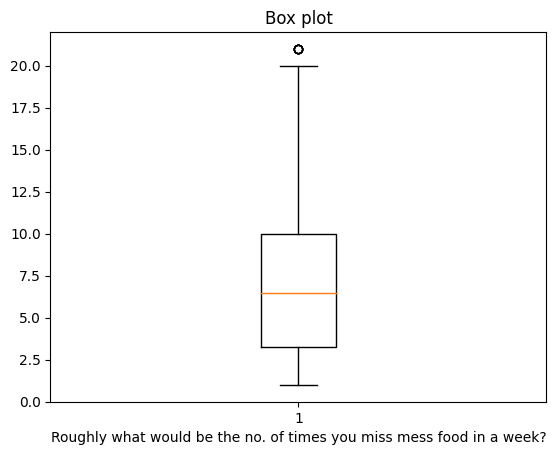
\includegraphics[scale = 1]{box_skipfrequency.png}
    \caption{Roughly what would be the no.of times you miss mess food in a week? (Box plot)}  
    \label{fig:boxplot}
\end{figure}
We can observe from the box plot that the plot of frequency would be slightly right skewed with median
around 6 (times a person missing a meal during a week), with the 1 outlier(greater than 20). The IQR is around
7.
\begin{figure}[H]
    \centering
    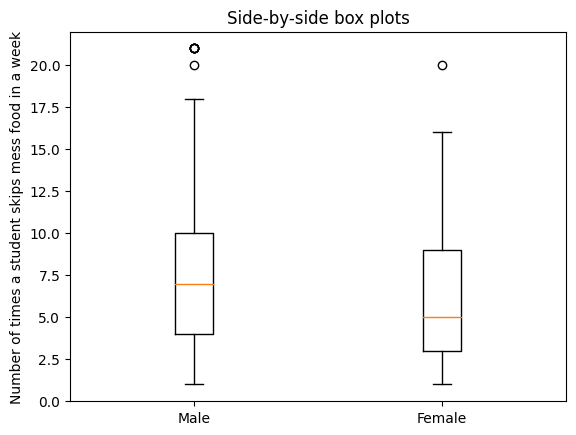
\includegraphics[scale = 0.9]{side-by-side-gender-skip-relation.png}
    \caption{Week-days vs Week-ends (Side-by-Side Box plot)}  
    \label{fig:side-by-side}
\end{figure}
Normal Probability Plot, which is used to assess whether the data is normally distributed or not, is given below:
\begin{figure}[H]
    \centering
    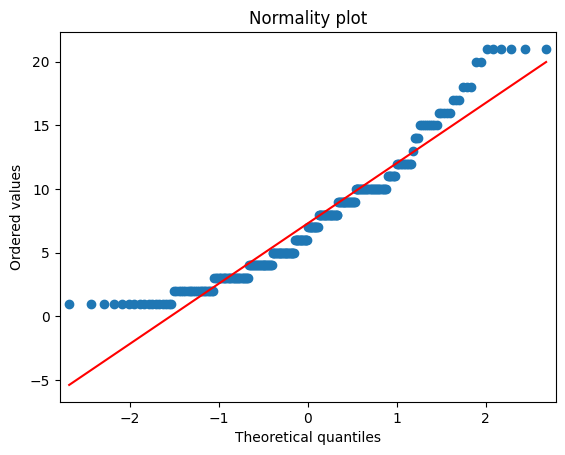
\includegraphics[scale = 0.9]{normality_plot.png}
    \caption{Normal Probability Plot}  
    \label{fig:Normality_plot}
\end{figure}

% ####################
\pagebreak
\centerline{\underline{\bfseries{ Degree vs number of responses}}}

% \centerline{I need to center align a {\bfseries word} with bold and underlines.}
\begin{figure}[H]
    \centering
    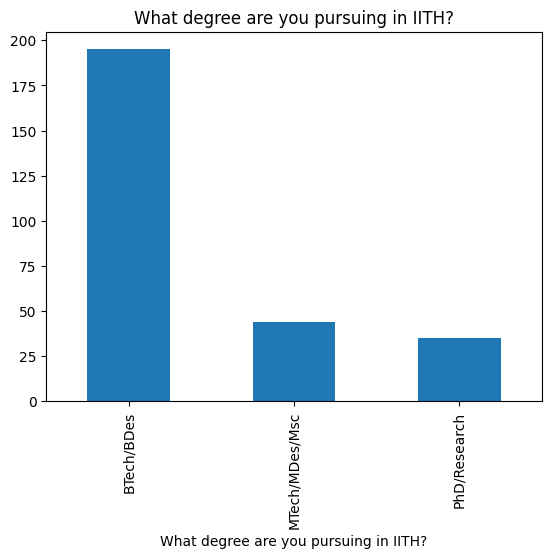
\includegraphics[scale = 0.7]{bar_degree.png}
    \caption{Degree vs number of responses bar graph}  
    \label{fig:Normality_plot}
\end{figure}
From this graph, we can see that students from BTech/Bdes responded the most for the contribution of data, which makes the analysis more centered around them.

% \pagebreak
\centerline{\underline{\bfseries{Branch vs number of responses}}}

\begin{figure}[H]
    \centering
    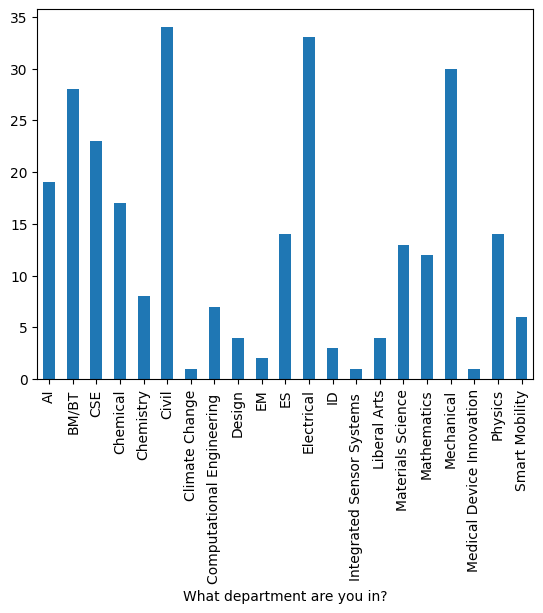
\includegraphics[scale = 0.6]{bar_department.png}
    \caption{Branches vs number of responses bar graph}  
    \label{fig:Normality_plot}
\end{figure}
This graph shows that the people who responded the most are from Civil, BM/BT, Mechanical \& Electrical.

\centerline{\underline{\bfseries{Share of different economic classes}}}

\begin{figure}[H]
    \centering
    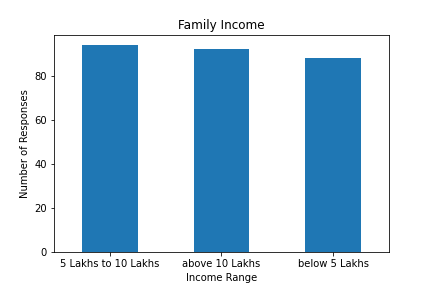
\includegraphics[scale = 0.7]{bar_familyincome.png}
    \caption{Family income bar graph}  
    \label{fig:Normality_plot}
\end{figure}
It is evident that all the three classes have almost equal share in our data.\\

% \pagebreak
\centerline{\underline{\bfseries{Which meal is being skipped the most?}}}
\begin{figure}[H]
    \centering
    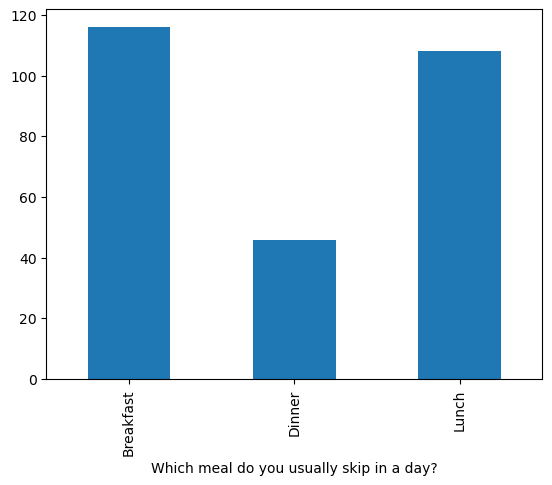
\includegraphics[scale = 0.7]{bar_timing_skip.png}
    \caption{Meal skip bar graph}
    \label{fig:Normality}
\end{figure}
From this bar graph, we can easily see that breakfast is being missed majorly by people (since many people work till late at night and wake up late in the morning). Lunch is also being missed by the majority of people (since maybe lunch is not good in the mess).\\

\pagebreak
\centerline{\underline{\bfseries{How many people skip meals and how many times?}}}
\begin{figure}[H]
    \centering
    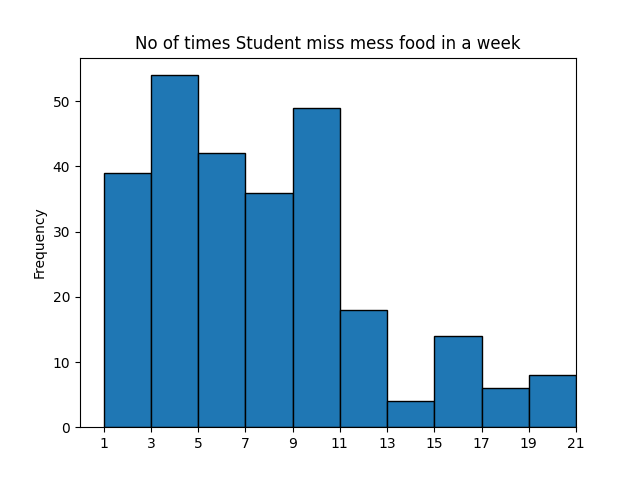
\includegraphics[scale = 0.7]{histogram_meal_skip.png}
    \caption{Frequecy of food missed vs Number of students}  
    \label{Normality_plot}
\end{figure}
From the histograms, it is evident that the plot is right-skewed, meaning that the people missing food more than 10 times a week are fewer. People mostly skip meals 2 to 7 times a week.
% \pagebreak

\centerline{\underline{\bfseries{Reasons for skipping a meal}}}

\begin{figure}[H]
    \centering
    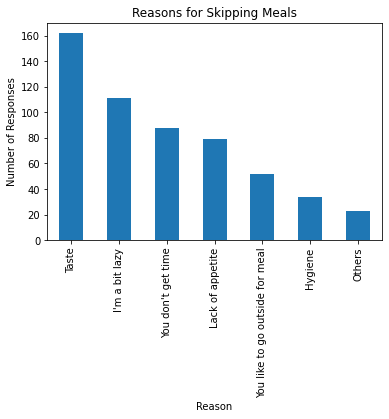
\includegraphics[scale = 0.7]{bar_reasons.png}
    \caption{Reasons vs frequency bar graph}  
    \label{fig:Normality_plot}
\end{figure}
We can easily observe that the most common reason of missing a particular meal is 'due to the bad taste of the food' being served. Other common reasons being 'I'm bit lazy', 'I don't get time', 'Like to go out for a meal' and others.
% \pagebreak

\centerline{\underline{\bfseries{Correlation of meal skipping with family income}}}

\begin{figure}[H]
    \centering
    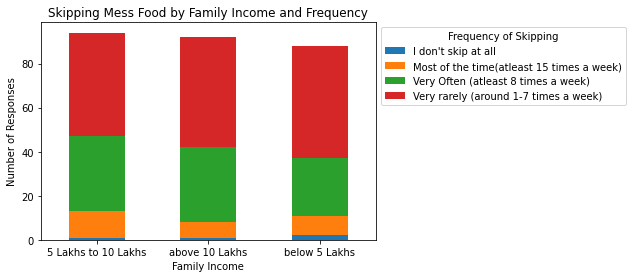
\includegraphics[scale = 0.7]{Meal Skipping - Family Income Seg chart.png}
    \caption{Skip meal-Family income segmented bar chart}  
    \label{fig:Normality_plot}
\end{figure}
It is evident that the meal skipping by the people is not very strongly correlated with their family income (we are getting similar bar charts for each economic class).\\

\centerline{\underline{\bfseries{Correlation of meal skipping with gender}}}

\begin{figure}[H]
    \centering
    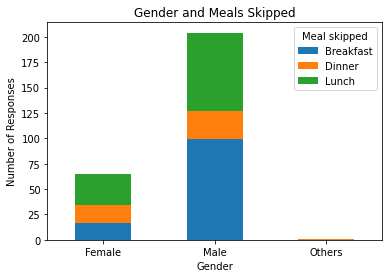
\includegraphics[scale = 0.7]{Meal Skipping - Gender Seg chart.png}
    \caption{Skip meal-Gender segmented bar chart}  
    \label{fig:Normality_plot}
\end{figure}
First of all it is clearly evident that the number of males who skip meals are around 3 times the number of females who skip meals (during a week) this is probably because less females(24\%) filled the form compared to males(76\%). In females all the three meals are being equally skipped (lunch having slight upper hand). In males breakfast is being skipped the most, followed by lunch. Dinner is not missed much by both males and females.
\pagebreak

\centerline{\underline{\bfseries{Reasons for skipping the meal}}}

\begin{figure}[H]
    \centering
    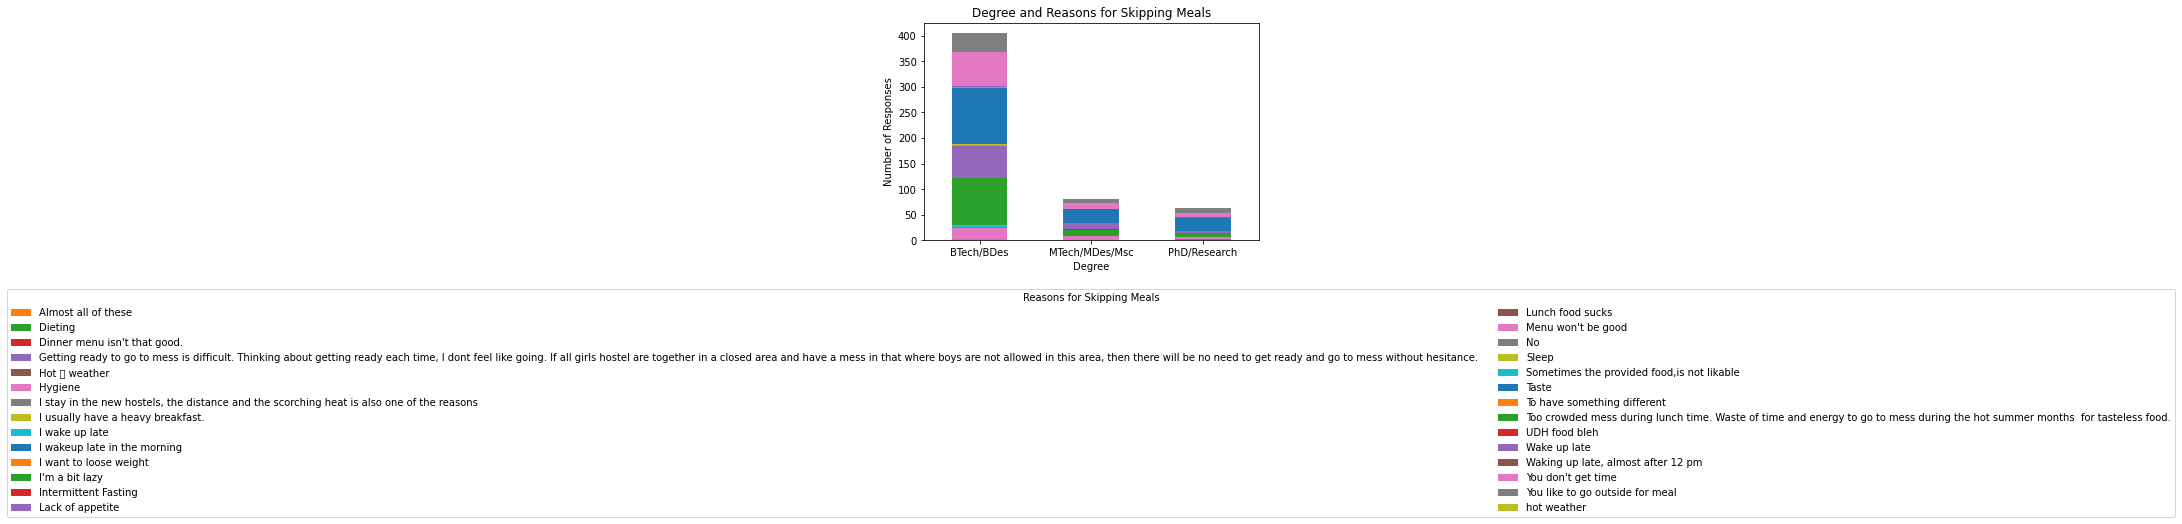
\includegraphics[scale = 0.7]{Meal Skipping - Reason Seg chart.png}
    \caption{Skip meal-Reason segmented bar chart}  
    \label{fig:Normality_plot}
\end{figure}
Here we can see that the BTech/Bdes responded the most. Secondly among the UGs the most common reason to be observed of missing a meal is 'taste of the food and laziness', with some other less common reasons being, 'hygiene', 'lack of appetite', 'do not have time', etc. For Non-UGs the most common reason being 'taste of the food' and least common reson being 'hygiene'.\\

\centerline{\underline{\bfseries{Correlation of sleep with missing meals}}}

\begin{figure}[H]
    \centering
    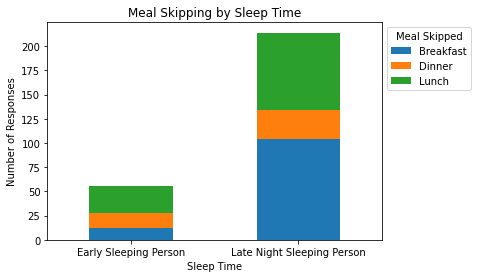
\includegraphics[scale = 0.7]{Meal Skipping - Sleep time Seg chart.png}
    \caption{Skip meal-Sleep segmented bar charts}  
    \label{fig:Normality_plot}
\end{figure}
It is clearly evident that the late night sleepers miss their meals the most. They clearly miss out on breakfasts followed by lunch, dinner is being missed out the least (both early and late night sleepers). Early sleeping people do not miss their meals regularly.

\pagebreak

\centerline{\underline{\bfseries{We will have a look on some pie charts now}}}

\begin{figure}[H]
    \centering
    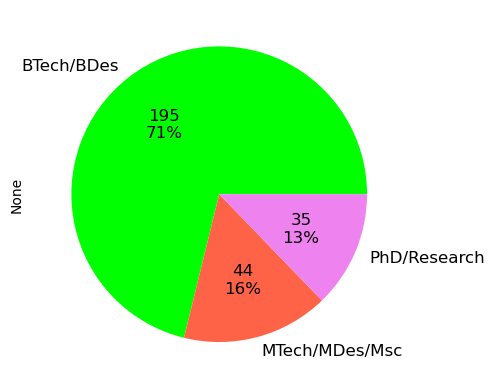
\includegraphics[scale = 0.9]{pie_degree.png}
    \caption{Degree at IITH pie chart}  
    \label{Normality_plot}
\end{figure}
Clearly evident that most of the respondents are from Btech/Bdes.

\begin{figure}[H]
    \centering
    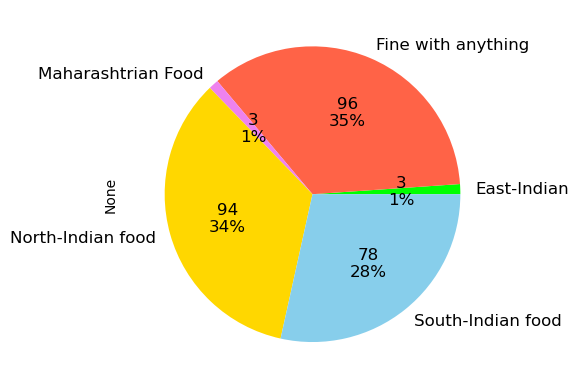
\includegraphics[scale = 0.9]{pie_food_pref.png}
    \caption{Food preference pie chart}  
    \label{Normality_plot}
\end{figure}
This pie chart shows the regional food preferences of the people in IITH. We can observe that people are not very particular about their food preferences.
\begin{figure}[H]
    \centering
    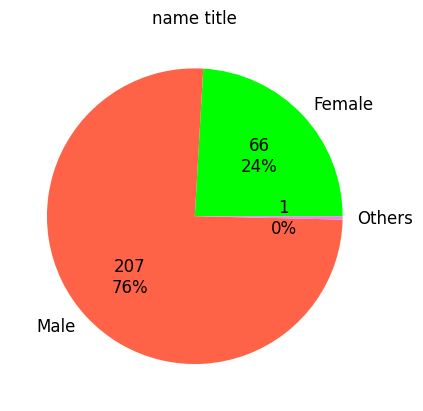
\includegraphics[scale = 0.9]{pie_gender.png}
    \caption{Gender Split}  
    \label{Normality_plot}
\end{figure}
The charts compare male to female responses. we see that nearly one-third of the total responses came from males
\begin{figure}[H]
    \centering
    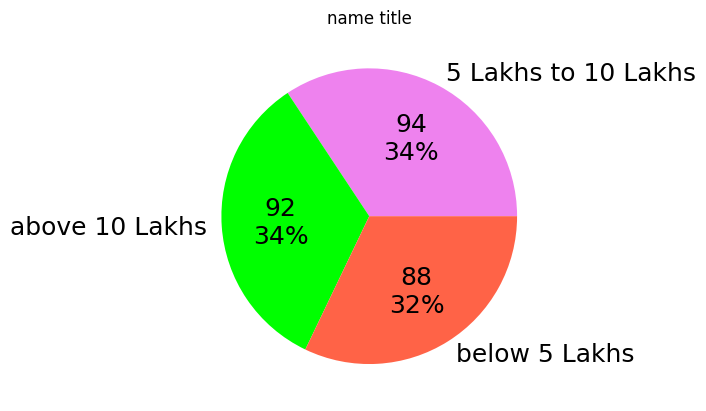
\includegraphics[scale = 0.9]{pie_income.png}
    \caption{Student's Family Income}  
    \label{Normality_plot}
\end{figure}
The chart shows the distribution of different economic classes in the responses. We can observe that it is very well balanced.
\begin{figure}[H]
    \centering
    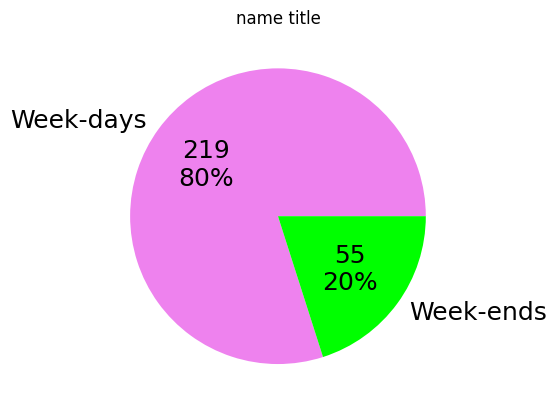
\includegraphics[scale = 0.9]{pie_plot_weekdays.png}
    \caption{Skipping meals on weekends or weekdays}  
    \label{Normality_plot}
\end{figure}
The pie chart above gives a comparison of skipping meals on weekends vs weekdays. We see the majority of skipping on weekdays. This may be because of specials on weekends.
\begin{figure}[H]
    \centering
    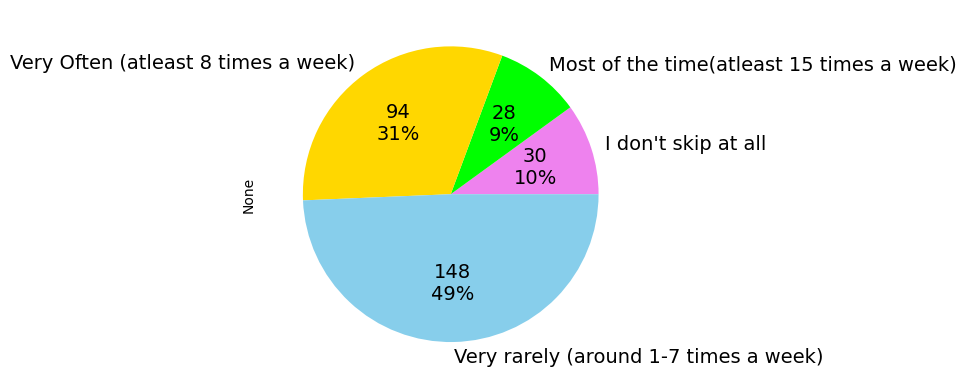
\includegraphics[scale = 0.75]{pie_skip_categoty.png}
    \caption{Frequency of missing food}  
    \label{Normality_plot}
\end{figure}
This pie chart compares the frequency of meal skipping. We find that half of the people rarely miss a meal.\\\\
\begin{figure}[H]
    \hspace{-22mm}% 
    \centering
    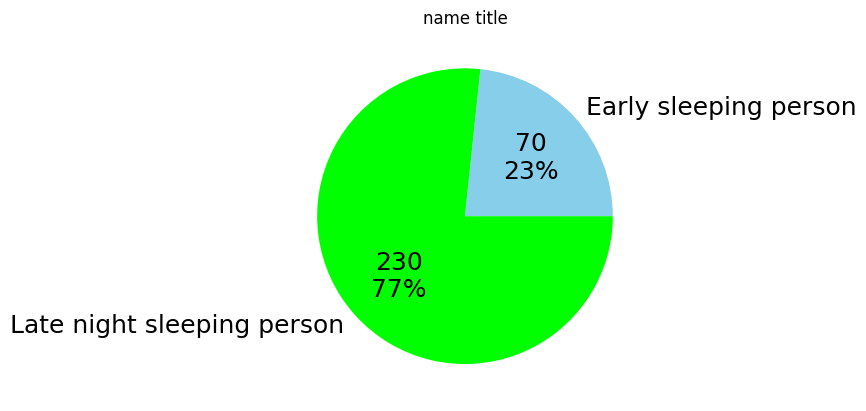
\includegraphics[scale = 0.75]{pie_sleep_categoty.png}
    \caption{Students are early sleepers or late nighters}  
    \label{Normality_plot}
\end{figure}
This pie chart compares Early sleepers vs Late sleepers in the responses. From this chart, we can infer that most are Late sleepers!!
% \centerline{\underline{\bfseries{Veg Vs}}}
\begin{figure}[H]
    \centering
    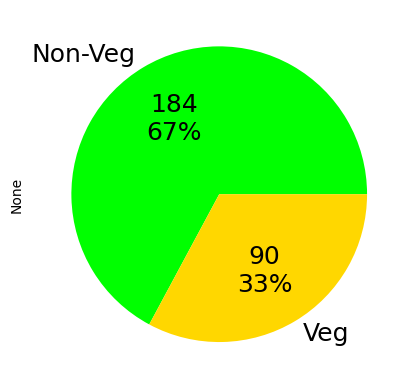
\includegraphics[scale = 0.9]{pie_veg_non-veg.png}
    \caption{Vegetarian vs Non-Vegetarian}  
    \label{Normality_plot}
\end{figure}
This pie chart compares Non-veg eaters vs veg eaters in the responses. From this chart, we can infer that there are 2 times as non-veg eaters as veg eaters!!

% \pagebreak
\bigskip
\section{Confidence Interval Estimation of Mean and Variance of the data.}
\begin{itemize}
    \item \textbf{Case-1: Confidence Interval of $\mu$, where $\mu$ is the mean number of meals skipped by a student at IITH in a week. } \\
       Consider a random sample of size $n = 50$. 
       Sample mean and sample standard deviation are $\bar{x}$ and $S$ respectively\\
        \begin{align*}
            \bar{x}&= 6.98 \\
            S &= 4.18 
        \end{align*}       
      
Also, for a $95\%$ CI, $\alpha=0.05$,$t_{\alpha/2,n-1} =t_{0.025,49}=2.0096$ \\
Now, the resulting $95\%$ CI is:
      \begin{align*}
        \bar{x}-t_{\alpha/2,n-1}\left(\frac{S}{\sqrt{n}}\right) &\leq \mu \leq \bar{x}+t_{\alpha/2,n-1}\left(\frac{S}{\sqrt{n}}\right)\\
        5.792 &\leq \mu \leq 8.168
      \end{align*}
      Thus, based on the sample data, the CI of the mean number of meals skipped by a student in a week is $[5.792,8.168]$\\
    \item \textbf{Case-2: Confidence Interval of $\sigma$,where $\sigma$ is the standard deviation of the population.} \\
       Consider a random sample of size $n = 50$.   \\
       Here sample variance,    $S^2 = 17.49$  \\
       Take, significance level $\alpha$ = 0.05                
        \begin{align*}
            &a = \chi^{2}_{1-\alpha/2,n-1} = \chi^{2}_{0.975,49} =67.505 \\
            &b = \chi^{2}_{\alpha/2,n-1} = \chi^{2}_{0.025,49} = 30.096
        \end{align*} 
        Now, the resulting $95\%$ CI is:
        \begin{align*}
            \frac{(n-1)S^2}{b} &\leq \sigma^2 \leq \frac{(n-1)S^2}{a}\\
            12.695 &\leq \sigma^2 \leq 28.476
          \end{align*}
          Thus,the obtained CI of $\sigma^2$ is $[12.695,28.476]$\\
          This leads to $95\%$ CI for $\sigma$ :$[3.563,5.336]$\\
\end{itemize}

\section{Hypothesis Testing}
\begin{itemize}
\item{\textbf{Case-1: Verifying if the mean count of students who skip mess during weekdays is greater than the mean count of the students who skip mess during week-ends with the level of significance 0.05.}}\\
Here, \\
Sample 1 is that of the students who skip mess during weekdays.\\
Sample 2 is that of the students who skip mess during weekends.
\begin{center}
Sample sizes : $n_1 = 216$ \quad $n_2 = 54$.
\end{center}
As both the sample sizes are greater than 30, The condition that population distributions are normal is satisfied.\\
Let's now declare the Null and Alternate Hypothesis\\
\textbf{$H_0$} : The mean count of students who skip mess during weekdays is less than or equal to that of students who skip mess during weekends.\\
\textbf{$H_a$} : The mean count of students who skip mess during weekdays is greater than that of students who skip mess during weekends.
\begin{center}
$H_0:\mu_1 - \mu_2 \leq 0$  vs  $H_a:\mu_1 - \mu_2 > 0$\\
Sample Means : $\bar{x_1} = 7.643  \quad \bar{x_2} = 5.907 $\\
Sample Variances : ${S_1}^2 = 23.396 \quad {S_2}^2 = 15.935$\\
\end{center}
Here, $\frac{{S_1}^2}{{S_2}^2} = 1.468$ which is less than 4. So, we can assume that both the variances are equal.
Let's now calculate the degrees of freedom and pooled variance:
\begin{center}
degrees of freedom $df = n_1 + n_2 - 2 = 268$\\
pooled variance ${S_p}^2 = \frac{\left(n_1-1\right){S_1}^2 + \left(n_2-1\right){S_2}^2}{df} = 21.92$
\end{center}
Test Statistic: :
\begin{center}
$t = \frac{\left(\bar{x_1}-\bar{x_2}\right) - D_0}{S_p\sqrt{\frac{1}{n_1}+\frac{1}{n2}}} = 0.5205$\\
\end{center}
\textbf{Rejection Region Approach :}Reject $H_o$ if $t \geq 1.6506$ where $t_{0.05,268} = 1.6506$ (here considered $\alpha = 0.05$).\\
\textbf{Result:} Because the observed value of t = 0.5205 is less than 1.6506 and hence is not in the rejection region, there is insufficient evidence to conclude that the mean count of students who skip mess during week-days is greater than the mean count of the students who skip mess during weekends.\\

\item{\textbf{Case-2: Verifying if the mean count of Undergraduate students who skip mess is different from 6 with 5\% as level of significance.}}\\
Here, the Sample is the Undergraduate students who skip mess.\\
Sample size n = 127.\\
Now, we set up the research hypotheses:\\
$H_0$ : Mean count of Undergraduate students who skip mess is 6.\\
$H_a$ : Mean count of Undergraduate students who skip mess differs from 6.
\begin{center}
$H_0 : \mu = 6$ \quad vs \quad $H_a : \mu \neq 6$\\
Sample Mean : $\bar{x} = 7.285$\\
Sample Standard deviation: $S = 4.572$
\end{center}
Test Statistic :
\begin{center}
$t^* = \frac{\bar{x}-\mu_0}{S/\sqrt{n}} = \frac{7.285-6}{4.572/\sqrt{127}} = 3.1673$\\
degrees of freedom : $df = 127 - 1 = 126$ \\
Level of significance : $\alpha = 0.05$
\end{center}
\textbf{p-value Approach:}
Since $H_a$ is two-tailed,
\begin{center}
$p-value = 2\times P(t>|t^*|) = 2\times P(t>|3.1673|)$ 
\end{center}
Since we do not find the exact value of 3.1673 in the t-table at 126 d.f., we try to find a range. It can be seen from the t-table that the value falls between 3.1562 and 3.1892, and corresponding to them, the right tail probabilities are 0.001 and 0.0009, respectively.\\
$\therefore$ The p-value would be between 2 × (0.0009) = 0.0018 and 2 × (0.001) = 0.002.\\
\textbf{Result:}
Since p-value is less than $\alpha$, there is significant evidence that the mean count of Undergraduate students who skip mess is different from 7.\\

\item{\textbf{Case-3: Verifying if the variability in count of students of age 19-20 years who skip mess is less than 7 with 0.05 as the level of significance.}}\\
Here, Sample is the 19-20 years age students who skip mess.
Let's now declare the null and alternative hypothesis,\\
$H_0$ : Variability in count of students of age 19-20 years who skip mess is greater than or equal to 7.\\
$H_a$ : Variability in count of students of age 19-20 years who skip mess is less than 7.
\begin{center}
$H_0 : \sigma^2 \geq 7$ vs $H_a : \sigma^2 < 7$\\
Sample size n = 124\\
Sample Variance : $S^2$ = 16.497
\end{center}
Test Statistic:
\begin{center}
$\chi^2 = \frac{(n-1){S^2}}{{\sigma_0}^2} = \frac{123\times16.497}{49} = 41.4108$
\end{center}
\textbf{Rejection region Approach:} 
Reject $H_0$ if the value of TS is less than 149.8846, for df = n-1 = 123 and $1 - \alpha = 0.95$.\\
\textbf{Result:}
Since the computed value 41.4108 is less than the critical value of 149.8846, there is sufficient evidence to reject $H_0$ i.e.; there is significant evidence that the variability in count of students of age 19-20 years who skip mess is less than 7.\\

\item{\textbf{Case-4: Verifying if the percentage of AI and CSE students who skip mess is greater than 0.1 with level of significance 0.05.}}\\
Here, Sample is the count of AI and CSE department students who skip mess.\\
Declaring null and alternate hypothesis,\\
$H_0$ : Percentage of AI and CSE department students who skip mess is less than or equal to 0.1.\\
$H_a$ : Percentage of AI and CSE department students who skip mess is greater than 0.1.
\begin{center}
$H_0 : \pi \leq 0.1$ vs $H_a : \pi > 0.1$\\
sample size n = 41
\end{center}
Test Statistic :
\begin{center}
$Z = \frac{\hat{\pi}-{\pi_0}}{\sigma_{\hat{\pi}}}$
\end{center}
From the survey data,\\
$\hat{\pi} = \frac{41}{270} = 0.1518$ and $\sigma_{\hat{\pi}} = \sqrt{\frac{0.1518(1-0.1518)}{270}} = 0.0218$\\
Also, 
\begin{center}
$n(\pi_0) = 270(0.155) = 40.986 > 5$ and $n(1-\pi_0) = 270(1-0.155) = 229.014 > 5.$
\end{center}
Thus, the sample considered is valid and we obtain :
\begin{center}
$Z = \frac{\hat{\pi}-{\pi_0}}{\sigma_{\hat{\pi}}} = \frac{0.1518-0.1}{0.0218} = 2.3761$
\end{center}
\textbf{Rejection Region Approach:}
Reject $H_0$ if $Z>1.645$ for $\alpha = 0.05$\\
\textbf{Result:}
Since the observed value of Z exceeds the critical value of
1.645, we conclude there is significant evidence that the
percentage of AI and CSE department students who skip mess exceeds the percentage of 10\%.

\end{itemize}

\section{Contributions}
\begin{enumerate}
\item Blessy Anvitha J
\begin{itemize}
  \item Ideation of the project
  \item Data Collection
  \item Hypothesis Testing 
  \item LATEX report on Hypothesis Testing
\end{itemize}
\item Saanvi Amrutha
\begin{itemize}
  \item Data Collection
  \item Central Tendencies of entire Sample
  \item Normality-plot, Box plots and Confidence Intervals
  \item LATEX report
\end{itemize}
\item Bhanu Prasad
\begin{itemize}
  \item Data Cleaning
  \item Data Pre-Processing for coding
  \item Python Coding for generating bar-charts and pie-charts
\end{itemize}
\item Anirudh Srinivasan
\begin{itemize}
  \item Idea of the Project
  \item Python Coding
\end{itemize}
\item Lokesh Surana
\begin{itemize}
  \item Data Collection
  \item Python Coding
  \item LATEX Report
\end{itemize}

\item Arnav Asati
\begin{itemize}
  \item Slides of Data Visualisation
  \item Results and Analysis
  \item Remaining LATEX report
\end{itemize}
\item Samar Singhai 
\begin{itemize}
  \item Slides of Data Visualisation
  \item Results and Analysis
  \item LATEX Report
\end{itemize}
\item Shivanand
\begin{itemize}
  \item Results and Analysis
  \item LATEX report
\end{itemize}
\end{enumerate}
\end{document} 